\documentclass[a4paper, 16pt]{article}
\usepackage[utf8]{inputenc}
\usepackage[english, russian]{babel} 
\usepackage[left=20mm, top=20mm, right=20mm,
 bottom=20mm, head=1mm, foot=1mm]{geometry}
\usepackage{tikz} 
\usepackage{amsmath, amsfonts, amssymb}
\usepackage{graphicx}
\usepackage{fancybox, fancyhdr}
\usepackage{hyperref}
\usepackage{listings}
\usepackage{caption}
\usepackage{xcolor}
\usepackage{subcaption}
\pagestyle{fancy}
\fancyhf{}
\fancyhead[L]{Лабораторная работа №2}
\fancyhead[R]{Техническое зрение}
\fancyfoot[C]{\thepage}
\graphicspath{{images/}}
\usetikzlibrary{patterns}
\definecolor{LightGray}{gray}{0.95}
\lstdefinestyle{pycode}{
    language=Python,
    basicstyle=\footnotesize\ttfamily,
    numbers=left,
    numberstyle=\tiny\color{gray},
    stepnumber=1,
    numbersep=5pt,
    backgroundcolor=\color{LightGray},
    showspaces=false,
    showstringspaces=false,
    showtabs=false,
    tabsize=4,
    captionpos=b,
    breaklines=true,
    breakatwhitespace=false,
    frame=none, % single
    framexleftmargin=-1mm,
    framexrightmargin=-1mm,
    rulecolor=\color{black},
    linewidth=\linewidth,
    keywordstyle=\color{red}\bfseries,
    commentstyle=\color{green!40!black},
    stringstyle=\color{blue},
    escapeinside={\%*}{*)},
    xleftmargin=0pt,
    framexleftmargin=0pt,
    framexrightmargin=0pt
}
\lstset{style=pycode}
\hypersetup{
    colorlinks=true,
    linkcolor=blue,
    filecolor=magenta,      
    urlcolor=cyan,
    pdftitle={contents setup},
    pdfpagemode=FullScreen,
}
\allowdisplaybreaks
\renewcommand{\lstlistingname}{Листинг}
\newcommand{\frc}[2]{\raisebox{2pt}{$#1$}\big/\raisebox{-3pt}{$#2$}}

\begin{document}
\begin{titlepage}

\begin{center}
\vfill

Федеральное государственное автономное образовательное учреждение высшего образования\\
«Национальный Исследовательский Университет ИТМО»\ \\

\vfill
{\large\bf ЛАБОРАТОРНАЯ РАБОТА №2\\
    ПО ПРЕДМЕТУ «ТЕХНИЧЕСКОЕ ЗРЕНИЕ»\\
    ПО ТЕМЕ «ГЕОМЕТРИЧЕСКИЕ ПРЕОБРАЗОВАНИЯ ИЗОБРАЖЕНИЙ»}\ \\
        
\vfill
    
\begin{flushright}
    \begin{minipage}{.45\textwidth}
        {
        \hbox{Преподаватель:}
        \hbox{Шаветов С. В.}
        \hbox{}
        \hbox{Выполнили:}
        \hbox{Румянцев А. А.}
        \hbox{Овчинников П. А.}
        \hbox{Чебаненко Д. А.}
        \hbox{}
        \hbox{Факультет: СУиР}
        \hbox{Группа: R3241}
        \hbox{Поток: ТЕХ.ЗРЕНИЕ 2.1}
        }
    \end{minipage}
\end{flushright}
        
\vfill
        
Санкт-Петербург\\
2024
\end{center}
\end{titlepage}
\setlength{\parskip}{1.5mm}


\tableofcontents


\newpage
\section{Начало}
\subsection{Цель}
\noindent Цель выполнения данной работы заключается в освоении основных видов отображений
и использовании геометрических преобразований для решения задач пространственной коррекции изображений


\subsection{Немного о преобразовании изображений}
\noindent Геометрические преобразования являются матричными преобразованиями. Множества
координат пикселей преобразованного и исходного изображений связаны следующим матричным
соотношением:
\begin{align*}
    X^{\prime}=XT\Rightarrow
    \begin{bmatrix}
        x^{\prime}\\
        y^{\prime}\\
        \omega^{\prime}
    \end{bmatrix}=
    \begin{bmatrix}
        A &B &C\\
        D &E &F\\
        G &H &I
    \end{bmatrix}\cdot
    \begin{bmatrix}
        x\\
        y\\
        \omega
    \end{bmatrix},
\end{align*}
\noindent где $X=\left(x,\,y,\,\omega\right)$ -- представление точки $X=\left(x,\,y\right)$ на
плоскости в двумерном пространстве $P^2$, $\omega$ -- скалярный произвольный множитель,
$x=\frc{x^{\prime}}{\omega},\,y=\frc{y^{\prime}}{\omega}$. Точка с декартовыми координатами
$\left(x,\,y\right)$ в однородных координатах примет вид $\left(x,\,y,\,1\right)$. Тогда:
\begin{align*}
    \begin{bmatrix}
        x^{\prime}\\
        y^{\prime}\\
        1
    \end{bmatrix}=
    \begin{bmatrix}
        A &B &C\\
        D &E &F\\
        0 &0 &1
    \end{bmatrix}\cdot
    \begin{bmatrix}
        x\\
        y\\
        1
    \end{bmatrix},
\end{align*}
\noindent что можно записать в виде следующей системы:
$$
\begin{cases}
    x^{\prime}=Ax+By+C\\
    y^{\prime}=Dx+Ey+F
\end{cases}
$$


\subsection{Оригинальная картинка}
Для всех исследуемых преобразований была выбрана следующая картинка:
\begin{figure}[!htb]
    \centering
    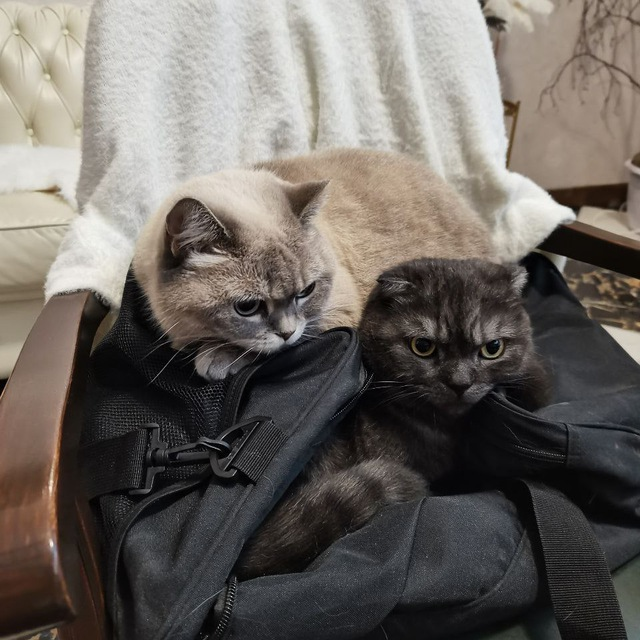
\includegraphics[scale=0.3]{img1.jpg}
    \captionsetup{skip=0pt}
    \caption{Оригинальная картинка}
    \label{Рис:1}
\end{figure}


\subsection{Язык программирования и необходимая библиотека}
\noindent Работа выполнена на языке программирования Python с использованием библиотеки OpenCV. Следующий 
код позволяет считать картинку в переменную и после сохранить изображение в заданную папку:
\begin{lstlisting}[label=start-code,caption=Пример использования библиотеки OpenCV на python]
import cv2

path = 'tech-vision/source/img1.jpg'
render_dir = 'tech-vision/renders/'

source_img = cv2.imread(path)
cv2.imwrite(f'{render_dir}cats.png', source_img)
\end{lstlisting}


\noindent На выходе получим картинку, приведенную на рисунке 1. В дальнейшем по умолчанию будут использоваться
переменные path, render\_{dir} и source\_{img}, но для экономии места каждый раз они приводиться не будут. Также подключим
библиотеку numpy для работы с матрицами преобразования


\section{Простейшие геометрические преобразования}
\subsection{Сдвиг изображения}
\noindent Сдвиг изображения -- это такое преобразование изображения, при котором все точки
картинки перемещаются в заданном направлении на заданное расстояние. Это преобразование можно
описать матрицей преобразования координат $T$, в которой в случае сдвига изображения $A=E=1,\,B=D=0$.
Ранее описанная система и матрица $T$ примут следующий вид:
$$
\begin{cases}
    x^{\prime}=x+C\\
    y^{\prime}=y+D
\end{cases}\,\,\,\,\,
T=
\begin{bmatrix}
    1 &0 &0\\
    0 &1 &0\\
    C &F &1
\end{bmatrix},
$$
\noindent где $C \text{ и } F$ -- сдвиг по осям $Ox \text{ и } Oy$ соответственно


\begin{lstlisting}[label=shift-code,caption=Код для сдвига изображения на 50 и 100 пикселей по осям $Ox \text{ и } Oy$]
import numpy as np

def shift_img(img, delta_x, delta_y):
    rows, cols = img.shape[0:2]
    t = np.float32([[1, 0, delta_x], [0, 1, delta_y]])
    return cv2.warpAffine(img, t, (cols, rows))

shifted_img = shift_img(source_img, delta_x=50, delta_y=100)
cv2.imwrite(f'{render_dir}shifted_img.png', shifted_img)
\end{lstlisting}


\begin{figure}[!htb]
    \centering
    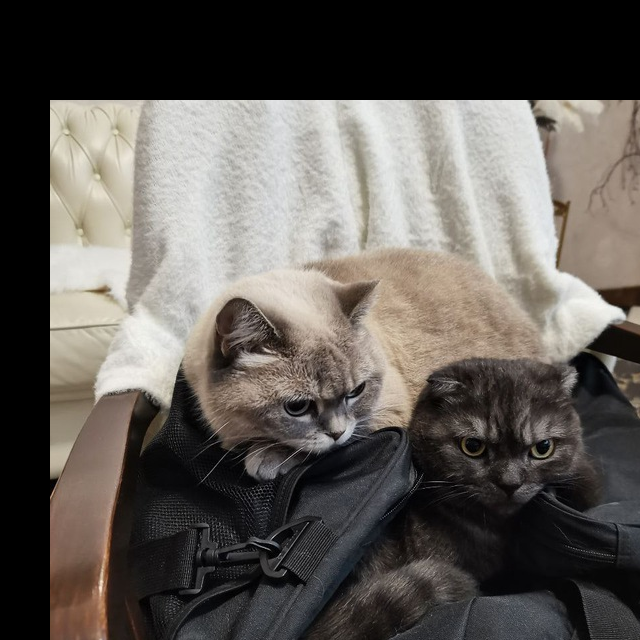
\includegraphics[scale=0.3]{shifted_img.png}
    \captionsetup{skip=0pt}
    \caption{Сдвиг изображения на 50 и 100 пикселей по осям $Ox \text{ и } Oy$ соответственно}
    \label{Рис:2}
\end{figure}


\noindent Как видим, изображение съехало больше по вертикали, чем по горизонтали, значит все
в порядке и оси координат не были перепутаны и написанный алгоритм выполнил свою задачу


\subsection{Отражение изображения}
\noindent Отражение изображения -- преобразование картинки, при котором каждый горизонтальный ряд
пикселей или каждый вертикальный ряд пикселей задается в обратном порядке относительно оригинального
изображения. Система уравнений из пункта 1.2 и матрица преобразования координат $T$ в случае отображения
изображения вдоль оси $Ox$ при $A=1,\,E=-1,\,B=C=D=F=0$ примут вид:
\begin{align*}
    \begin{cases}
        x^{\prime}=x\\
        y^{\prime}=-y
    \end{cases}\Rightarrow\,\,\,\,
    T=
    \begin{bmatrix}
        1 &0 &0\\
        0 &-1 &0\\
        0 &0 &1
    \end{bmatrix}
\end{align*}


\noindent Код ниже позволяет отражать изображение относительно оси $Ox$, если
параметр flag==true, в противном случае относительно оси $Oy$. Воспользуемся им для
получения двух новых картинок:
\begin{lstlisting}[label=reflect-code,caption=Код для отражения относительно оси $Ox \text{ или } Oy$]
def reflect_img(img, flag: bool):
    rows, cols = img.shape[0:2]
    if (flag):
        t = np.float32([[1, 0, 0], [0, -1, rows - 1]])
    else:
        t = np.float32([[-1, 0, rows - 1], [0, 1, 0]])
    return cv2.warpAffine(img, t, (cols, rows))

reflected_img_ox = reflect_img(source_img, flag=True)
reflected_img_oy= reflect_img(source_img, flag=False)
cv2.imwrite(f'{render_dir}reflect_img_ox.png', reflected_img_ox)
cv2.imwrite(f'{render_dir}reflect_img_oy.png', reflected_img_oy)
\end{lstlisting}


\begin{figure}[!htb]
    \centering
    \begin{minipage}{0.45\textwidth}
        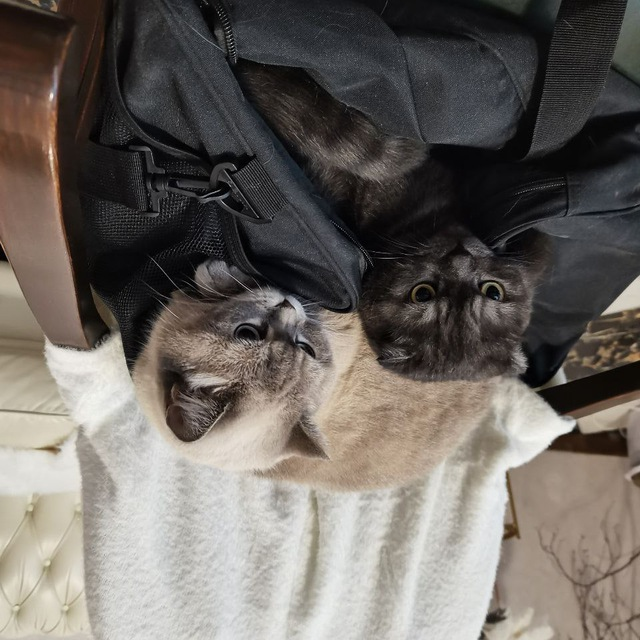
\includegraphics[scale=0.3]{reflect_img_ox.png}
        \captionsetup{skip=0pt}
        \caption{Отражение изображения относительно оси $Ox$}
        \label{Рис:3}
    \end{minipage}\hfill
    \begin{minipage}{0.45\textwidth}
        \centering
        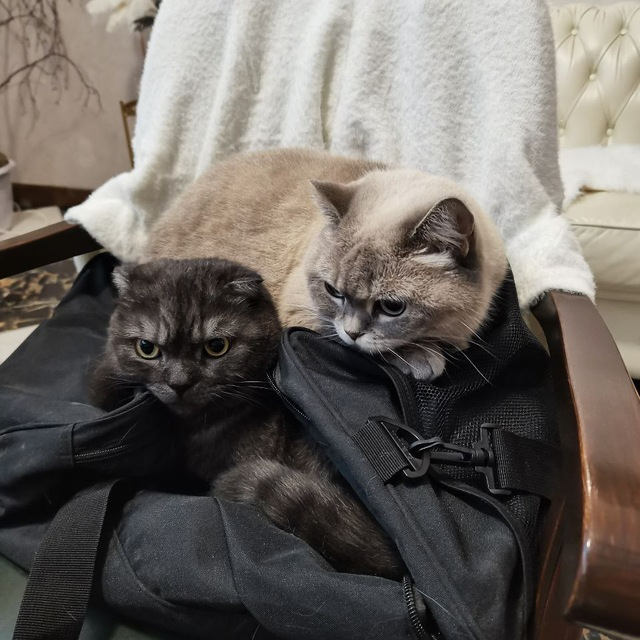
\includegraphics[scale=0.3]{reflect_img_oy.png}
        \captionsetup{skip=0pt}
        \caption{Отражение изображения относительно оси $Oy$}
        \label{Рис:4}
    \end{minipage}
\end{figure}


\subsection{Однородное масштабирование изображения}
\noindent Однородное масштабирование изображения -- такое матричное преобразование картинки,
при котором размеры изображения меняются с помощью увеличения или уменьшения его размеров
на одинаковый коэффициент по всем направлениям. Система уравнений из пункта 1.2 и матрица 
преобразования координат $T$ в данном случае $A=\alpha,\,E=\beta,\,B=C=D=F=0$ примут вид:
\begin{align*}
    \begin{cases}
        x^{\prime}=\alpha x,\,\alpha>0\\
        y^{\prime}=\beta y,\,\beta>0
    \end{cases}\Rightarrow\,\,\,\,
    T=
    \begin{bmatrix}
        \alpha &0 &0\\
        0 &\beta &0\\
        0 &0 &1
    \end{bmatrix}
\end{align*}


\noindent Если $\alpha<1 \text{ и } \beta<1$, то изображение уменьшается, если 
$\alpha>1 \text{ и } \beta>1$, то увеличивается. Если $\alpha\neq\beta$, то пропорции
будут не одинаковыми по ширине и высоте


\noindent В случае использования библиотеки OpenCV из матрицы $T$ пропадает последняя строчка.
Воспользуемся следующим кодом для масштабирования изображения:
\begin{lstlisting}[label=scale-code,caption=Код для масштабирования изображения]
def scale_img(img, scale_x, scale_y):
    rows, cols = img.shape[0:2]
    t = np.float32([[scale_x, 0, 0], [0, scale_y, 0]])
    return cv2.warpAffine(img, t, (int(cols * scale_x), int(rows * scale_y)))

scaled_img_bigger = scale_img(source_img, 2, 2)
scaled_img_smaller = scale_img(source_img, 0.5, 0.5)
scaled_img_wtf = scale_img(source_img, 1, 0.5)
cv2.imwrite(f'{render_dir}scaled_img_bigger.png', scaled_img_bigger)
cv2.imwrite(f'{render_dir}scaled_img_smaller.png', scaled_img_smaller)
cv2.imwrite(f'{render_dir}scaled_img_wtf.png', scaled_img_wtf)
\end{lstlisting}


\begin{figure}[!htb]
    \centering
    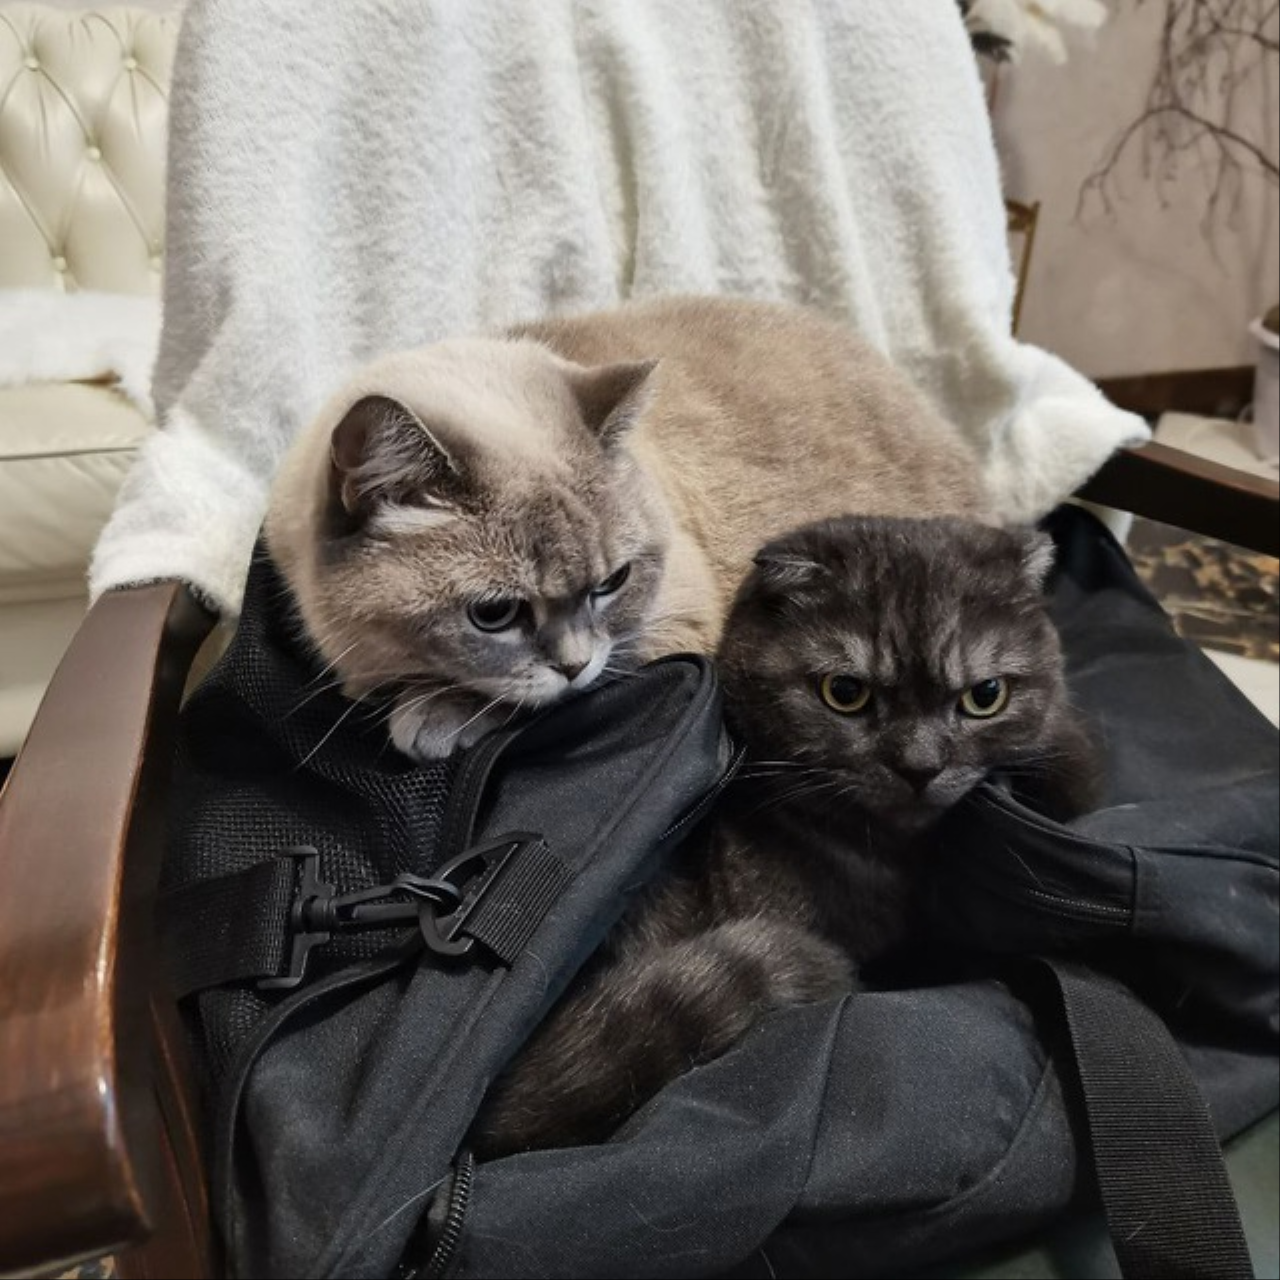
\includegraphics[scale=0.3]{scaled_img_bigger.png}
    \captionsetup{skip=0pt}
    \caption{Увеличенное в два раза изображение}
    \label{Рис:5}
\end{figure}


\begin{figure}[!htb]
    \centering
    \begin{minipage}{0.45\textwidth}
        \centering
        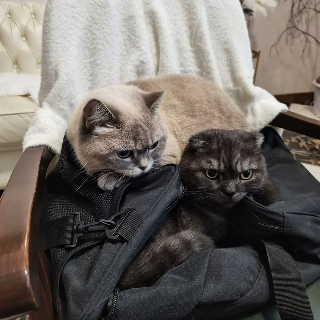
\includegraphics[scale=0.3]{scaled_img_smaller.png}
        \captionsetup{skip=0pt}
        \caption{Уменьшенное в два раза изображение}
        \label{Рис:6}
    \end{minipage}\hfill
    \begin{minipage}{0.45\textwidth}
        \centering
        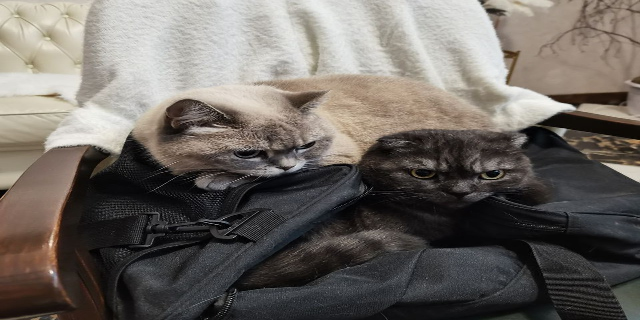
\includegraphics[scale=0.3]{scaled_img_wtf.png}
        \captionsetup{skip=0pt}
        \caption{Уменьшенное по высоте изображение}
        \label{Рис:7}
    \end{minipage}
\end{figure}


\noindent Кошки побольше, кошки поменьше и широкие кошки. Красота. А главное -- работает


\subsection{Поворот изображения}
\noindent Поворот изображения -- преобразование изображения, при котором картинка
вращается вокруг некоторой точки или оси на заданный угол. Система уравнений пункта 1.2
и матрица $T$ в случае поворота по часовой стрелке $A=\cos{\phi},\,B=-\sin{\phi},\,D=\sin{\phi},\,E=\cos{\phi},\,C=F=0$
примут вид:
\begin{align*}
    \begin{cases}
        x^{\prime}=x\cos{\phi}-y\sin{\phi}\\
        y^{\prime}=x\sin{\phi}+y\cos{\phi}
    \end{cases}\Rightarrow\,\,\,\,
    T=
    \begin{bmatrix}
        \cos{\phi} &\sin{\phi} &0\\
        -\sin{\phi} &\cos{\phi} &0\\
        0 &0 &1
    \end{bmatrix}
\end{align*}


\noindent В случае использования библиотеки OpenCV из матрицы $T$ пропадает последняя строчка.
Рассмотрим код ниже. Метод rotate\_{img} поворачивает изображение относительно левого верхнего угла картинки,
а метод rotate\_{img}\_{center} относительно центра:
\begin{lstlisting}[label=rotate-code,caption=Код для поворота изображения]
def rotate_img(img, angle):
    rows, cols = img.shape[0:2]
    phi = np.radians(angle)
    t = np.float32([[np.cos(phi), -np.sin(phi), 0], [np.sin(phi), np.cos(phi), 0]])
    return cv2.warpAffine(img, t, (cols, rows))

def rotate_img_center(img, angle):
    rows, cols = img.shape[0:2]
    phi = np.radians(angle)
    t1 = np.float32([[1, 0, -(cols - 1) / 2], [0, 1, -(rows - 1) / 2], [0, 0, 1]])
    t2 = np.float32([[np.cos(phi), -np.sin(phi), 0], [np.sin(phi), np.cos(phi), 0], [0, 0, 1]])
    t3 = np.float32([[1, 0, (cols - 1) / 2], [0, 1, (rows - 1) / 2], [0, 0, 1]])
    t = np.matmul(t3, np.matmul(t2, t1))[0:2, :]
    return cv2.warpAffine(img, t, (cols, rows))

rotated_img = rotate_img(source_img, angle=45)
cv2.imwrite(f'{render_dir}rotated_img.png', rotated_img)

rotated_img_center = rotate_img_center(source_img, angle=45)
cv2.imwrite(f'{render_dir}rotated_img_center.png', rotated_img_center)
\end{lstlisting}


\begin{figure}[!htb]
    \centering
    \begin{minipage}{0.45\textwidth}
        \centering
        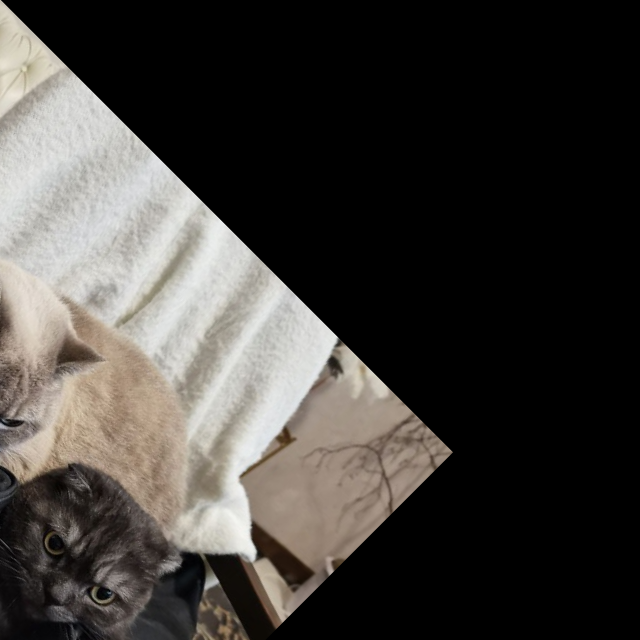
\includegraphics[scale=0.3]{rotated_img.png}
        \captionsetup{skip=0pt}
        \caption{Поворот изображения относительно левого угла на $45^{\circ}$}
        \label{Рис:8}
    \end{minipage}\hfill
    \begin{minipage}{0.45\textwidth}
        \centering
        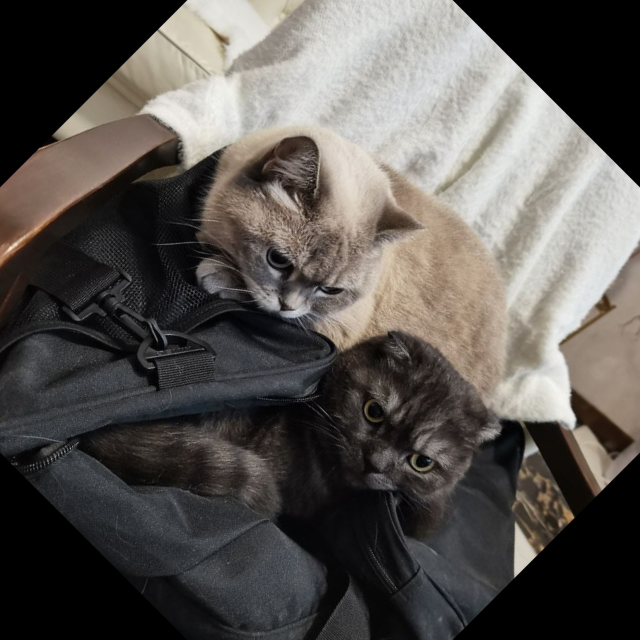
\includegraphics[scale=0.3]{rotated_img_center.png}
        \captionsetup{skip=0pt}
        \caption{Поворот изображения относительно центра на $45^{\circ}$}
        \label{Рис:9}
    \end{minipage}
\end{figure}


\subsection{Скос изображения}
\noindent Скос изображения -- такое преобразование картинки, при котором происходит
смещение всех точек вдоль одной из осей на заданное расстояние, причем стороны остаются
параллелльными, но углы между ними меняются. Система уравнений пункта 1.2 и матрица $T$
в данном случае $A=E=1,\,B=s,\,C=D=F=0$ примут вид:
\begin{align*}
    \begin{cases}
        x^{\prime}=x+sy\\
        y^{\prime}=y
    \end{cases}\Rightarrow\,\,\,\,
    T=
    \begin{bmatrix}
        1 &0 &0\\
        s &1 &0\\
        0 &0 &1
    \end{bmatrix}
\end{align*}


\newpage
\noindent Скос изображения с помощью кода на python с $s=0.3$:
\begin{lstlisting}[label=bevel-code,caption=Код для скоса изображения]
def bevel_img(img, arg):
    rows, cols = img.shape[0:2]
    t = np.float32([[1, arg, 0], [0, 1, 0]])
    return cv2.warpAffine(img, t, (cols, rows))

beveled_img = bevel_img(source_img, 0.3)
cv2.imwrite(f'{render_dir}beveled_img.png', beveled_img)
\end{lstlisting}


\begin{figure}[!htb]
    \centering
    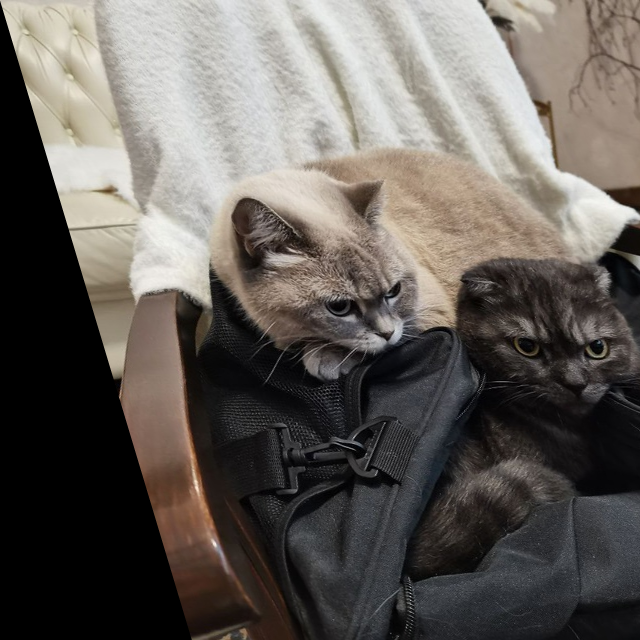
\includegraphics[scale=0.3]{beveled_img.png}
    \captionsetup{skip=0pt}
    \caption{Скос изображения}
    \label{Рис:10}
\end{figure}


\subsection{Кусочно-линейное отображение}
\noindent Кусочно-линейное отображение -- это отображение, при котором 
картинка разбивается на части, а после к каждой части применяются различные
линейные преобразования


\noindent Следующий код растягивает правую часть изображения вдоль оси $Ox$, а
левую оставляет без изменений
\begin{lstlisting}[label=piecewise-code,caption=Код для изменения правой части изображения по оси $Ox$]
def piecewise_linear_mapping(img, arg):
    rows, cols = img.shape[0:2]
    t = np.float32([[arg, 0, 0], [0, 1, 0]])
    img[:, int(cols / 2):, :] = cv2.warpAffine(img[:, int(cols / 2):, :], t, (cols - int(cols / 2), rows))
    return img

piecewiselinear2 = piecewise_linear_mapping(source_img, 2)
piecewiselinear05 = piecewise_linear_mapping(source_img, 0.5)
cv2.imwrite(f'{render_dir}piecewiselinear2.png', piecewiselinear2)
cv2.imwrite(f'{render_dir}piecewiselinear05.png', piecewiselinear05)
\end{lstlisting}


\newpage
\begin{figure}[!htb]
    \centering
    \begin{minipage}{0.45\textwidth}
        \centering
        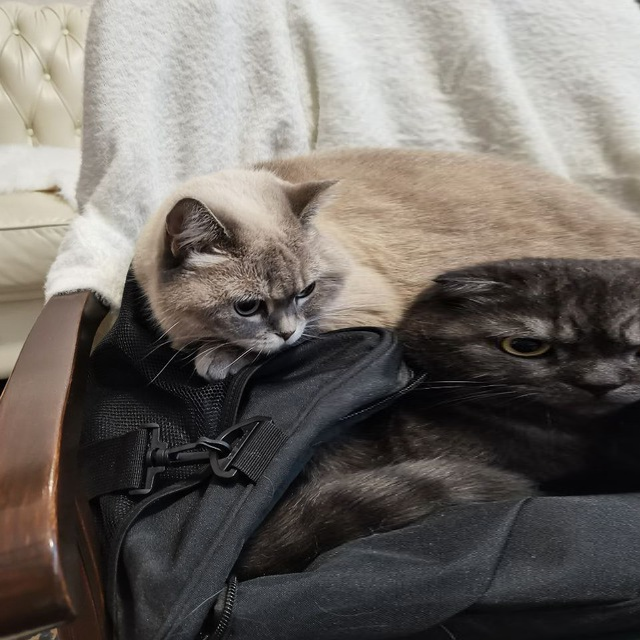
\includegraphics[scale=0.3]{piecewiselinear2.png}
        \captionsetup{skip=0pt}
        \caption{Растяжение правой части изображения вдоль оси $Ox$ в два раза}
        \label{Рис:11}
    \end{minipage}
    \begin{minipage}{0.45\textwidth}
        \centering
        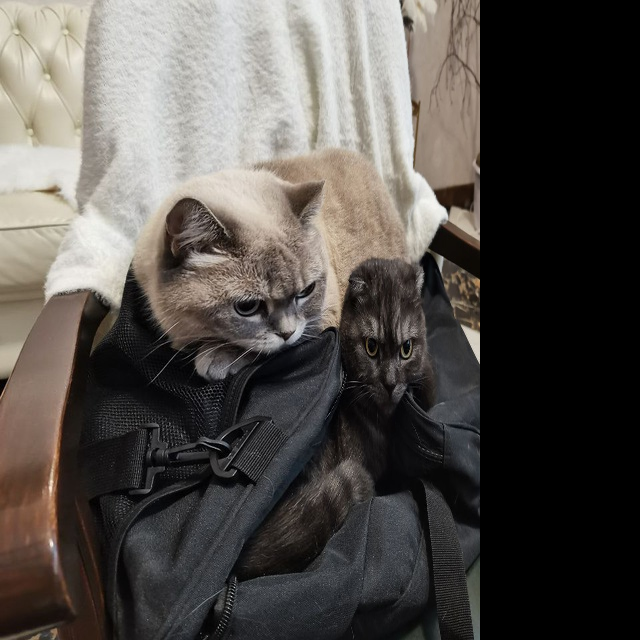
\includegraphics[scale=0.3]{piecewiselinear05.png}
        \captionsetup{skip=0pt}
        \caption{Сужение правой части изображения вдоль оси $Ox$ в два раза}
        \label{Рис:12}
    \end{minipage}
\end{figure}


\subsection{Проекционное отображение}
\noindent Проекционное отображение -- это отображение, при котором прямые линии
остаются прямыми линиями, однако геометрия фигуры может быть нарушена, так как 
данное отображение в общем случае не сохраняет параллелльности линий. Однако три точки,
лежащие на одной прямой (коллинеарные), после преобразования остаются на одной прямой.
Проекционное отображение может быть как параллелльным (изменение масштаба), так и 
проективными (изменение геометрии фигуры). Система и матрица преобразования $T$ в
таком случае примут вид:
\begin{align*}
    \begin{cases}
        x^{\prime}=\dfrac{Ax+By+C}{Gx+Hy+I}\\
        y^{\prime}=\dfrac{Dx+Ey+F}{Gx+Hy+I}
    \end{cases}\Rightarrow\,\,\,\,
    T=
    \begin{bmatrix}
        A &B &C\\
        D &E &F\\
        G &H &1
    \end{bmatrix}
\end{align*}


\noindent Пример кода, где $A=1.1,\,B=0.35,\,C=F=0,\,D=0.2,\,E=1.1,\,G=0.00075,\,H=0.0005,\,I=1$
\begin{lstlisting}[label=projection-code,caption=Код для проективного отображения]
def projection(img, arr):
    rows, cols = img.shape[0:2]
    t = np.float32(arr)
    return cv2.warpPerspective(img, t, (cols, rows))

projected_img = projection(source_img, [[1.1, 0.35, 0], [0.2, 1.1, 0], [0.00075, 0.0005, 1]])
cv2.imwrite(f'{render_dir}projected_img.png', projected_img)
\end{lstlisting}


\newpage
\begin{figure}[!htb]
    \centering
    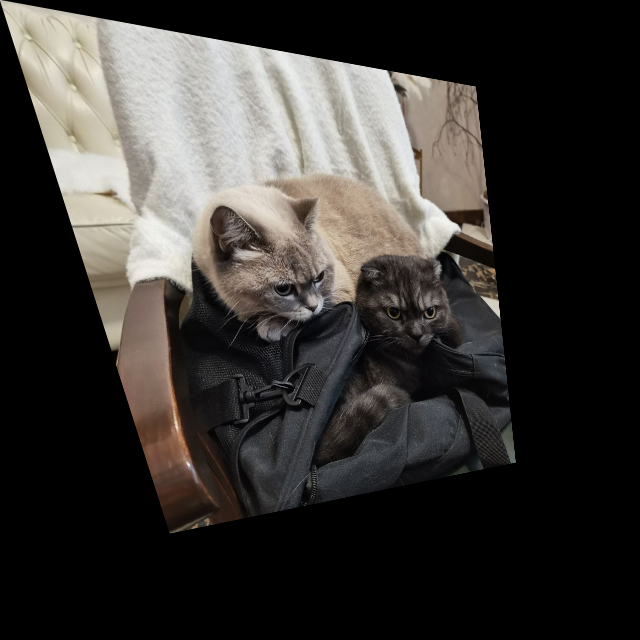
\includegraphics[scale=0.3]{projected_img.png}
    \captionsetup{skip=0pt}
    \caption{Проективное отображение}
    \label{Рис:13}
\end{figure}


\subsection{Полиномиальное отображение}
\noindent Полиномиальное отображение -- название говорит само за себя -- это
отображение исходного изображения с помощью полиномов. Матрица $T$ будет содержать
коэффициенты полиномов соответствующих порядков для координат $x \text { и } y$. В
случае полиномиального преобразования второго порядка система пункта 1.2 примет вид:
$$
\begin{cases}
    x^{\prime}=a_1+a_2x+a_3y+a_4x^2+a_5xy+a_6y^2\\
    y^{\prime}=b_1+b_2x+b_3y+b_4x^2+b_5xy+b_6y^2
\end{cases},
$$


\noindent где $x,\,y$ -- координаты точек в одной системе координат,
$x^{\prime},\,y^{\prime}$ -- координаты этих точек в другой системе координат,
$a_1\hdots a_6,\,b_1\hdots b_6$ -- коэффициенты преобразования


\noindent Результирующее образованное кодом ниже изображение не будет содержать интерполированных пикселей:
\begin{lstlisting}[label=polynomial-code,caption=Код для полиномиального отображения]
def polynomial(img, t):
    rows, cols = img.shape[0:2]
    t = np.array(t)
    I_polynomial = np.zeros(img.shape, img.dtype)

    x, y = np.meshgrid(np.arange(cols),
                       np.arange(rows))
    xnew = np.round(t[0, 0] + x * t[1, 0] +
                    y * t[2, 0] + x * x * t[3, 0] +
                    x * y * t[4, 0] +
                    y * y * t[5, 0]).astype(np.float32)
    ynew = np.round(t[0, 1] + x * t[1, 1] +
                    y * t[2, 1] + x * x * t[3, 1] +
                    x * y * t[4, 1] +
                    y * y * t[5, 1]).astype(np.float32)
    mask = np.logical_and(
        np.logical_and(xnew >= 0, xnew < cols),
        np.logical_and(ynew >= 0, ynew < rows))
    if img.ndim == 2:

        I_polynomial[ynew[mask].astype(int),

        xnew[mask].astype(int)] = \
            img[y[mask], x[mask]]
    else:
        I_polynomial[ynew[mask].astype(int),
        xnew[mask].astype(int), :] = \
            img[y[mask], x[mask], :]
    return I_polynomial

T = [[0, 0], [1, 0], [0, 1], [0.00001, 0], [0.002, 0], [0.001, 0]]
m = polynomial(source_img, T)
cv2.imwrite(f'{render_dir}polynomial.png', m)
\end{lstlisting}


\begin{figure}[!htb]
    \centering
    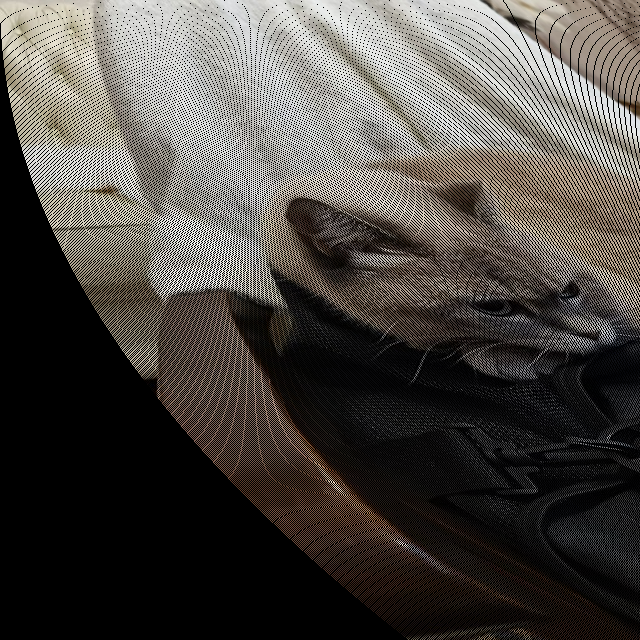
\includegraphics[scale=0.3]{polynomial.png}
    \captionsetup{skip=0pt}
    \caption{Полиномиальное отображение}
    \label{Рис:14}
\end{figure}


\subsection{Синусоидальное искажение}
\noindent Синусоидальное искажение -- гармоническое искажение картинки,
при котором пиксели перемещаются вверх и вниз или влево и вправо в зависимости
от позиции на изображении, что создает эффект волнистости или искривления


\begin{lstlisting}[label=sinusoidal-code,caption=Код для синусоидального искажения]
def sinusoidal(img):
    rows, cols = img.shape[0:2]
    u, v = np.meshgrid(np.arange(cols), np.arange(rows))
    u = u + 20 * np.sin(2 * np.pi * v / 90)
    img_sinusoid = cv2.remap(img, u.astype(np.float32), v.astype(np.float32), cv2.INTER_LINEAR)
    return img_sinusoid

sinusoid = sinusoidal(source_img)
cv2.imwrite(f'{render_dir}sinusoid.png', sinusoid)
\end{lstlisting}


\begin{figure}[!htb]
    \centering
    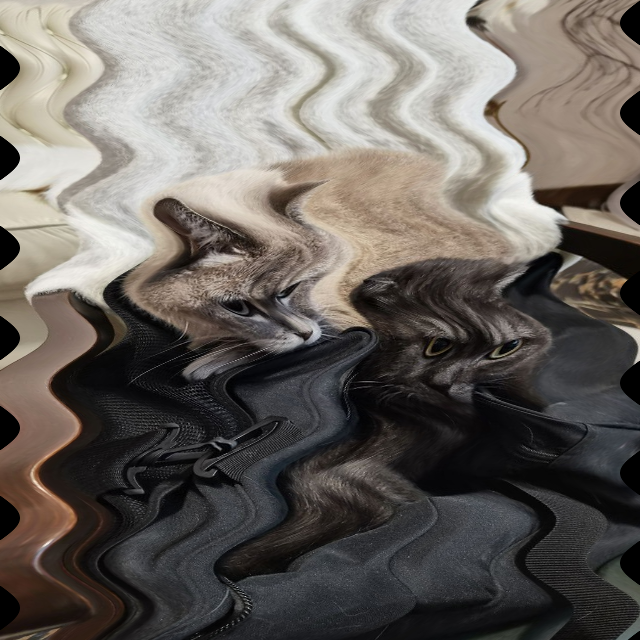
\includegraphics[scale=0.3]{sinusoid.png}
    \captionsetup{skip=0pt}
    \caption{Синусоидальное отображение}
    \label{Рис:15}
\end{figure}


\newpage
\subsection{Бочкообразная дисторсия}
\noindent Бочкообразная дисторсия -- отрицательная дисторсия --
оптическое искажение картинки, при котором объекты, находящиеся
ближе к краям, становятся сжатыми в направлении центра.
Пусть $\mathbf{r}=\left(x,\,y\right)$ -- вектор, задающий две координаты в плоскости,
расположенной перпенидкулярно оптической оси. Все лучи, вышедшие из этой точки и
прошедшие через оптическую систему, попадут в точку изображения с координатами $\mathbf{R}$,
которые в общем виде определяются по формуле:
\begin{align*}
    \mathbf{R}=b_0\mathbf{r}+F_3r^2\mathbf{r}+F_5r^4\mathbf{r}+\hdots,
\end{align*}


\noindent где $r$ -- длина вектора $\mathbf{r}$; $F_i,\,i=3,\,5,\,\hdots,\,n$ -- коэффициенты
дисторсии $n$-ого порядка, которые вносят наибольший вклад в искажение формы изображения


\begin{lstlisting}[label=barrel-code,caption=Код для бочкообразной дисторсии]
def barrel_distorsion(img):
    rows, cols = img.shape[0:2]
    xi, yi = np.meshgrid(np.arange(cols),
                         np.arange(rows))
    xmid = cols / 2.0
    ymid = rows / 2.0
    xi = xi - xmid
    yi = yi - ymid
    r, theta = cv2.cartToPolar(xi / xmid, yi / ymid)
    F3 = 0.1
    F5 = 0.12
    r = r + F3 * r ** 3 + F5 * r ** 5
    u, v = cv2.polarToCart(r, theta)
    u = u * xmid + xmid
    v = v * ymid + ymid
    I_barrel = \
        cv2.remap(img, u.astype(np.float32),
                  v.astype(np.float32), cv2.INTER_LINEAR)
    return I_barrel

barreled = barrel_distorsion(source_img)
cv2.imwrite(f'{render_dir}barrel.png', barreled)
\end{lstlisting}


\begin{figure}[!htb]
    \centering
    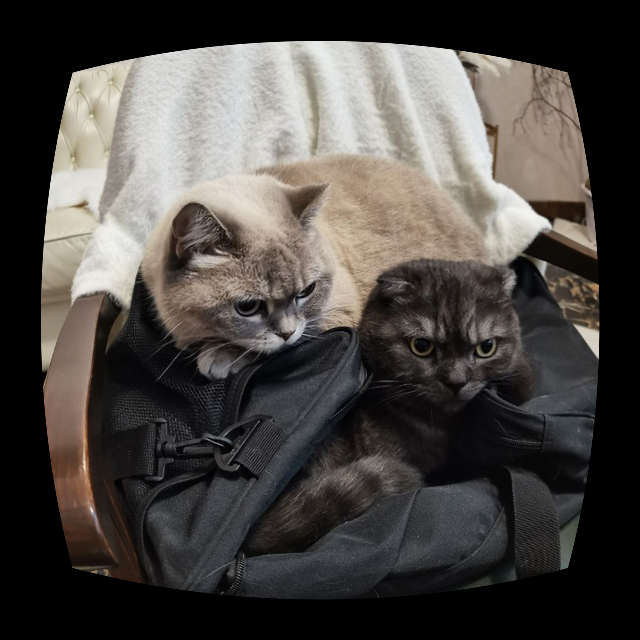
\includegraphics[scale=0.3]{barrel.png}
    \captionsetup{skip=0pt}
    \caption{Бочкообразная дисторсия}
    \label{Рис:16}
\end{figure}


\subsection{Подушкообразная дисторсия}
\noindent Подушкообразная дисторсия -- положительная дисторсия --
оптическое искажение картинки, при котором объекты, находящиеся ближе к 
центру изображения, кажутся уплощенными, а объекты, находящиеся ближе к краям,
кажутся выпуклыми или "надутыми". Формулы такие же, как в пункте 2.10


\newpage
\begin{lstlisting}[label=pincushion-code,caption=Код для подушкообразной дисторсии]
def pincushion_distorsion(img):
    rows, cols = img.shape[0:2]
    xi, yi = np.meshgrid(np.arange(cols),
                         np.arange(rows))
    xmid = cols / 2.0
    ymid = rows / 2.0
    xi = xi - xmid
    yi = yi - ymid
    r, theta = cv2.cartToPolar(xi / xmid, yi / ymid)
    F3 = -0.1
    F5 = -0.12
    r = r + F3 * r ** 3 + F5 * r ** 5
    u, v = cv2.polarToCart(r, theta)
    u = u * xmid + xmid
    v = v * ymid + ymid
    I_barrel = \
        cv2.remap(img, u.astype(np.float32),
                  v.astype(np.float32), cv2.INTER_LINEAR)
    return I_barrel

p = pincushion_distorsion(source_img)
cv2.imwrite(f'{render_dir}pil_distort.png', p)
\end{lstlisting}


\begin{figure}[!htb]
    \centering
    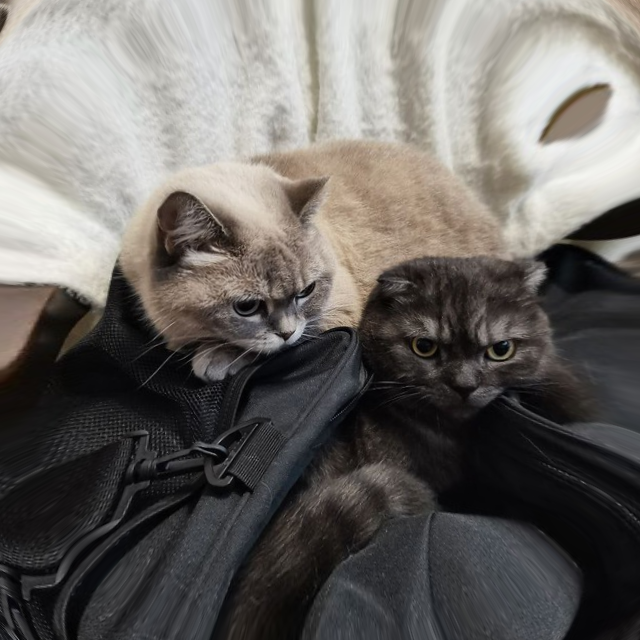
\includegraphics[scale=0.3]{pil_distort.png}
    \captionsetup{skip=0pt}
    \caption{Подушкообразная дисторсия}
    \label{Рис:17}
\end{figure}


\newpage
\section{Коррекция дистории}
\noindent Для коррекции дисторсии используется подход
для проективного отображения. Используется изображение
регулярной сетки и его искаженное изображение, находятся
пары точек на этих изображениях и вычисляются коэффициенты
корректирующего преобразования. Возьмем два искаженных изображения
и его оригинал:
\begin{figure}[!htb]
    \centering
    \begin{subfigure}[b]{0.3\textwidth}
        \centering
        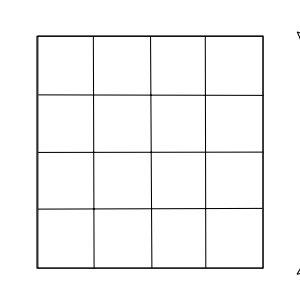
\includegraphics[width=\textwidth]{orig.png}
        \caption{Оригинальное изображение}
        \label{fig:original}
    \end{subfigure}
    \hfill
    \begin{subfigure}[b]{0.3\textwidth}
        \centering
        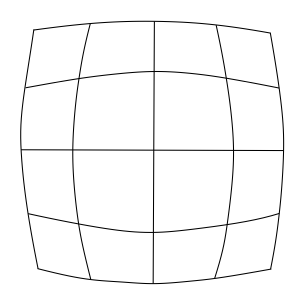
\includegraphics[width=\textwidth]{barbarrel.png}
        \caption{Бочкообразная дистория}
        \label{fig:barreled}
    \end{subfigure}
    \hfill
    \begin{subfigure}[b]{0.3\textwidth}
        \centering
        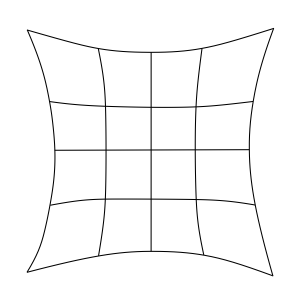
\includegraphics[width=\textwidth]{pipillow.png}
        \caption{Подушкообразная дистории}
        \label{fig:pillowed}
    \end{subfigure}
    \caption{Изображения для последующей коррекции и сравнения}
    \label{fig:origbarpil}
\end{figure}


\subsection{Коррекция бочкообразной дисторсии}
\noindent Попробуем починить бочку подушкой этой программой:
\begin{lstlisting}[label=fixbarr-code,caption=Код для коррекции бочкообразной дисторсии]
def undistort_barrel(img):
    rows, cols = img.shape[0:2]
    xi, yi = np.meshgrid(np.arange(cols), np.arange(rows))
    xmid = cols / 2.0
    ymid = rows / 2.0
    xi = xi - xmid
    yi = yi - ymid
    r, theta = cv2.cartToPolar(xi / xmid, yi / ymid)

    F3 = 0.1
    F5 = 0.06

    r = r - F3 * r ** 3 - F5 * r ** 5  # Apply the inverse distortion
    u, v = cv2.polarToCart(r, theta)
    u = u * xmid + xmid
    v = v * ymid + ymid

    I_undistorted = cv2.remap(img, u.astype(np.float32), v.astype(np.float32), cv2.INTER_LINEAR,
                              borderMode=cv2.BORDER_CONSTANT, borderValue=(255, 255, 255))

    return I_undistorted

barreled = barrel_distorsion(source_img)
undistort_bar = undistort_barrel(barreled)
cv2.imwrite(f'{render_dir}undistort_bar.png', undistort_bar)
\end{lstlisting}


\newpage
\begin{figure}[!htb]
    \centering
    \begin{minipage}{0.45\textwidth}
        \centering
        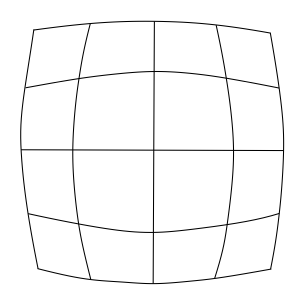
\includegraphics{barbarrel.png}
        \captionsetup{skip=0pt}
        \caption{Бочкообразная дисторсия}
        \label{Рис:18}
    \end{minipage}
    \begin{minipage}{0.45\textwidth}
        \centering
        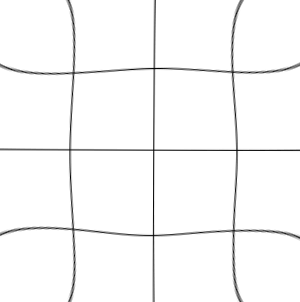
\includegraphics[scale=0.5]{undistort_bar.png}
        \captionsetup{skip=0pt}
        \caption{Коррекция бочки подушкой}
        \label{Рис:19}
    \end{minipage}
\end{figure}


\noindent Потеряли контур изображения, линии получились извилистые,
однако мы получили что-то отдаленно напоминающее оригинал


\subsection{Коррекция подушкообразной дисторсии}
\noindent Сыграем в бочку, подушку и оригинальное изображение следующим кодом и узнаем,
бьет ли бочка подушку:
\begin{lstlisting}[label=fixpin-code,caption=Код для коррекции подушкообразной дисторсии]
def undistort_pincushion(img):
    rows, cols = img.shape[0:2]
    xi, yi = np.meshgrid(np.arange(cols),
                         np.arange(rows))
    xmid = cols / 2.0
    ymid = rows / 2.0
    xi = xi - xmid
    yi = yi - ymid
    r, theta = cv2.cartToPolar(xi / xmid, yi / ymid)
    F3 = 0.5
    F5 = 1
    r = r + F3 * r ** 3 + F5 * r ** 5
    u, v = cv2.polarToCart(r, theta)
    u = u * xmid + xmid
    v = v * ymid + ymid
    I_barrel = \
        cv2.remap(img, u.astype(np.float32),
                  v.astype(np.float32), cv2.INTER_LINEAR)
    return I_barrel

p = pincushion_distorsion(source_img)
undistort_pin = undistort_pincushion(p)
cv2.imwrite(f'{render_dir}undistort_pin.png', undistort_pin)
\end{lstlisting}


\begin{figure}[!htb]
    \centering
    \begin{minipage}{0.45\textwidth}
        \centering
        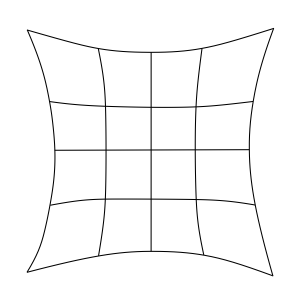
\includegraphics{pipillow.png}
        \captionsetup{skip=0pt}
        \caption{Подушкообразная дисторсия}
        \label{Рис:20}
    \end{minipage}
    \begin{minipage}{0.45\textwidth}
        \centering
        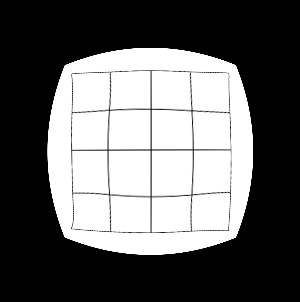
\includegraphics[scale=0.5]{undistort_pin.png}
        \captionsetup{skip=0pt}
        \caption{Коррекция подушки бочкой}
        \label{Рис:21}
    \end{minipage}
\end{figure}


\noindent Изображение стало куда хуже выглядеть -- потерялось качество
и размер, но мы добились похожести на оригинал хоть в каком то виде


\section{<<Склейка>> изображений}
\noindent <<Склейка>> изображений -- объединение двух или более
изображений в единое целое, причем системы координат склеиваемых
изображений могут отличаться из-за разного ракурса съемки, изменения
положения камеры или движения самого объекта. Однако необходимо, чтобы
оба изображения имели области перекрытия, то есть на них присутствовали
одинаковые объекты. Основной задачей обработки таких изображений является
введение их в общую систему координат. Для пересчета координат в случае 
афинного отображения система 1.2 примет вид:
$$
\begin{cases}
    x^{\prime}=a_1+a_2x+a_3y\\
    y^{\prime}=b_1+b_2x+b_3
\end{cases}
$$
\noindent Поэтому необходимо найти лишь по 3 коэффициента преобразования по каждой координате:
\begin{align*}
    &\begin{bmatrix}
        a_1\\
        a_2\\
        a_3
    \end{bmatrix}=
    \begin{bmatrix}
        1 &x_1 & y_1\\
        1 &x_2 &y_2\\
        1 &x_3 &y_3
    \end{bmatrix}^{-1}
    \begin{bmatrix}
        x_1^{\prime}\\
        x_2^{\prime}\\
        x_3^{\prime}
    \end{bmatrix}\\
    &\begin{bmatrix}
        b_1\\
        b_2\\
        b_3
    \end{bmatrix}=
    \begin{bmatrix}
        1 &x_1 & y_1\\
        1 &x_2 &y_2\\
        1 &x_3 &y_3
    \end{bmatrix}^{-1}
    \begin{bmatrix}
        y_1^{\prime}\\
        y_2^{\prime}\\
        y_3^{\prime}
    \end{bmatrix}
\end{align*}


\noindent Для этого на обоих изображениях следует
выбрать соответствующие пары точек (три пары в случае
аффинного искажения и не менее шести пар в случае полиномиального искажения).
Будем рассматривать простой случай «склейки» двух неискаженных изображений,
имеющих одинаковую ширину. Необходимо склеить их по вертикали, то есть
добавить к первому второе снизу. Однако, граница склейки неизвестна.
Эту задачу можно реализовать при помощи корреляционного подхода


\subsection{Ручная склейка изображения}
\noindent Разделим кошек пополам по горизонтали:
\begin{figure}[!htb]
    \centering
    \begin{minipage}{0.45\textwidth}
        \centering
        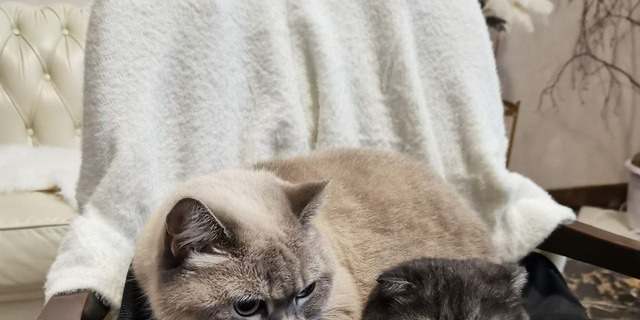
\includegraphics[scale=0.3]{top.jpg}
        \captionsetup{skip=0pt}
        \caption{Верхняя часть изображения}
        \label{Рис:22}
    \end{minipage}
    \begin{minipage}{0.45\textwidth}
        \centering
        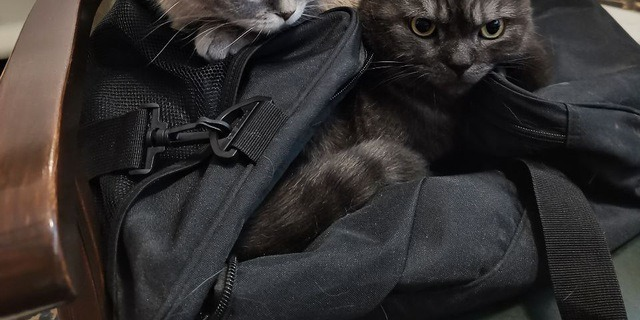
\includegraphics[scale=0.3]{bot.jpg}
        \captionsetup{skip=0pt}
        \caption{Нижняя часть изображения}
        \label{Рис:23}
    \end{minipage}
\end{figure}


\begin{lstlisting}[label=join-code,caption=Код для склейки верхней части изображения с нижней]
def join_img(topPart, botPart):
    templ_size = 10
    templ = topPart[- templ_size:, :, :]
    res = cv2.matchTemplate(botPart, templ,
    cv2.TM_CCOEFF )
    min_val, max_val, min_loc, max_loc = cv2.minMaxLoc(res)
    result_img = np.zeros(( topPart . shape [0] + botPart . shape [0] - max_loc [1]
                            - templ_size , topPart . shape [1] , topPart . shape [2]) , dtype = np . uint8 )
    result_img[0: topPart.shape[0], :, :] = topPart
    result_img[topPart.shape[0]:, :, :] = botPart [ max_loc [1] + templ_size : , : , :]
    return result_img

f_part = cv2.imread('tech-vision/source/top.jpg', cv2.IMREAD_COLOR)
s_part = cv2.imread('tech-vision/source/bot.jpg', cv2.IMREAD_COLOR)

ans = join_img(f_part, s_part)
cv2.imwrite(f'{render_dir}join.png', ans)
\end{lstlisting}


\newpage
\begin{figure}[!htb]
    \centering
    \begin{minipage}{0.45\textwidth}
        \centering
        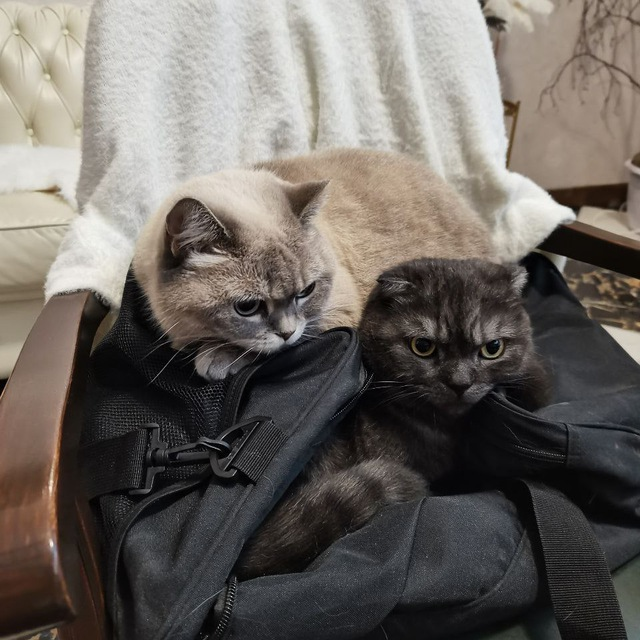
\includegraphics[scale=0.3]{img1.jpg}
        \captionsetup{skip=0pt}
        \caption{Оригинальное изображение}
        \label{Рис:24}
    \end{minipage}
    \begin{minipage}{0.45\textwidth}
        \centering
        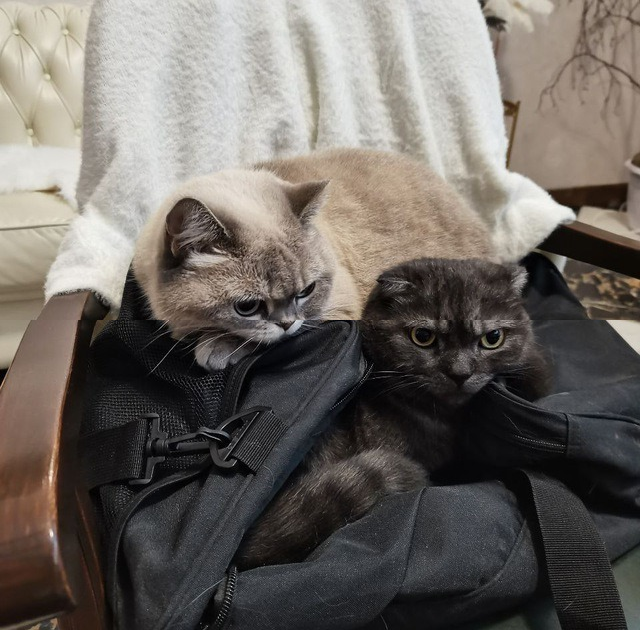
\includegraphics[scale=0.3]{join.png}
        \captionsetup{skip=0pt}
        \caption{Кошачье воссоединение}
        \label{Рис:25}
    \end{minipage}
\end{figure}


\noindent Почти идеально -- в месте соединения некоторые детали потерялись


\subsection{Автоматическая склейка изображения}
\noindent Всё то же самое, только теперь будем использовать класс Stitcher библиотеки OpenCV.
Разделим кошек по вертикали на три части:
\begin{figure}[!htb]
    \centering
    \begin{subfigure}[b]{0.3\textwidth}
        \centering
        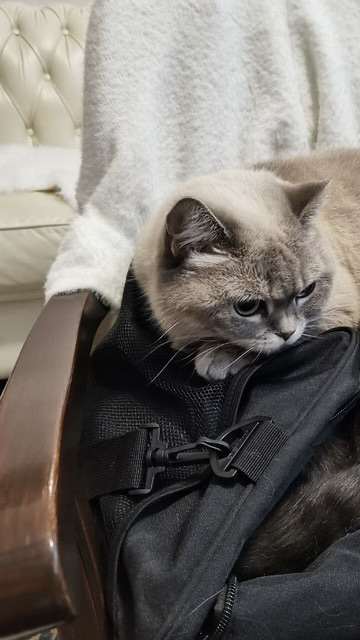
\includegraphics[width=\textwidth]{I1.jpg}
        \caption{Левая часть}
        \label{fig:left}
    \end{subfigure}
    \hfill
    \begin{subfigure}[b]{0.3\textwidth}
        \centering
        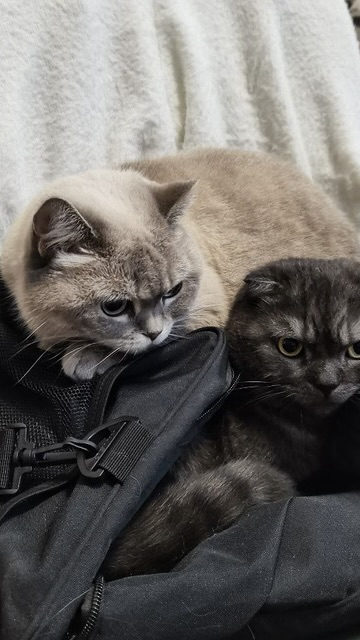
\includegraphics[width=\textwidth]{I2.jpg}
        \caption{Центральная часть}
        \label{fig:center}
    \end{subfigure}
    \hfill
    \begin{subfigure}[b]{0.3\textwidth}
        \centering
        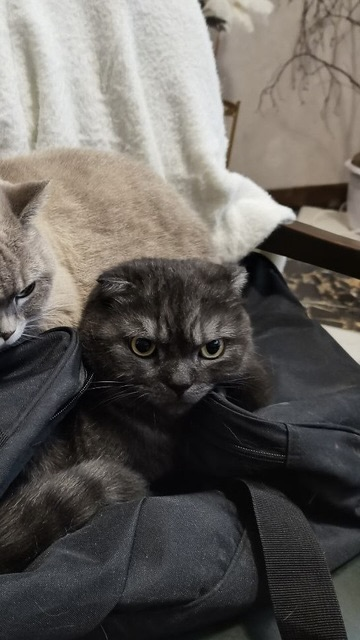
\includegraphics[width=\textwidth]{I3.jpg}
        \caption{Правая часть}
        \label{fig:right}
    \end{subfigure}
    \caption{Три части оригинального изображения}
    \label{fig:three_images}
\end{figure}


\begin{lstlisting}[label=aujoin-code,caption=Код для автоматической склейки изображений]
def auto_join_img(imgs:list):
    stitcher = cv2.Stitcher.create(cv2.Stitcher_PANORAMA)
    status, I_stitch = stitcher.stitch(imgs)
    return status, I_stitch

I_3 = cv2.imread('tech-vision/source/I1.jpg', cv2.IMREAD_COLOR)
I_2 = cv2.imread('tech-vision/source/I2.jpg', cv2.IMREAD_COLOR)
I_1 = cv2.imread('tech-vision/source/I3.jpg', cv2.IMREAD_COLOR)
status, I_stitch = auto_join_img([I_1, I_2, I_3])
cv2.imwrite(f'{render_dir}auto_join.png', I_stitch)
\end{lstlisting}


\begin{figure}[!htb]
    \centering
    \begin{minipage}{0.45\textwidth}
        \centering
        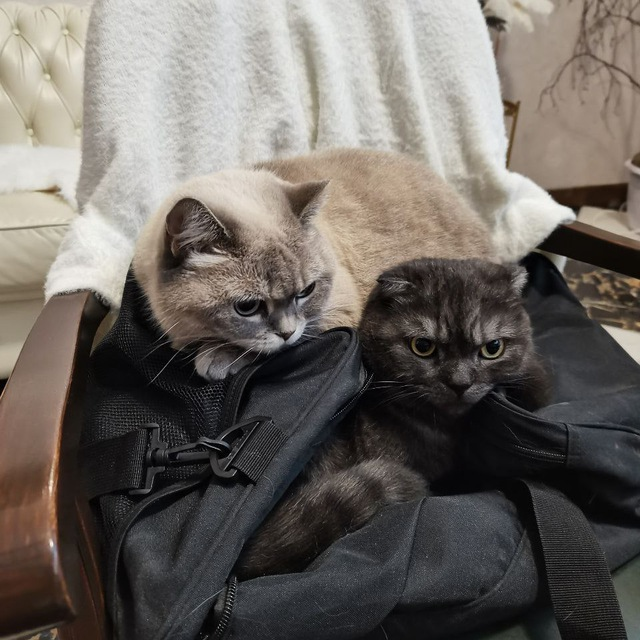
\includegraphics[scale=0.3]{img1.jpg}
        \captionsetup{skip=0pt}
        \caption{Оригинальное изображение}
        \label{Рис:27}
    \end{minipage}
    \begin{minipage}{0.45\textwidth}
        \centering
        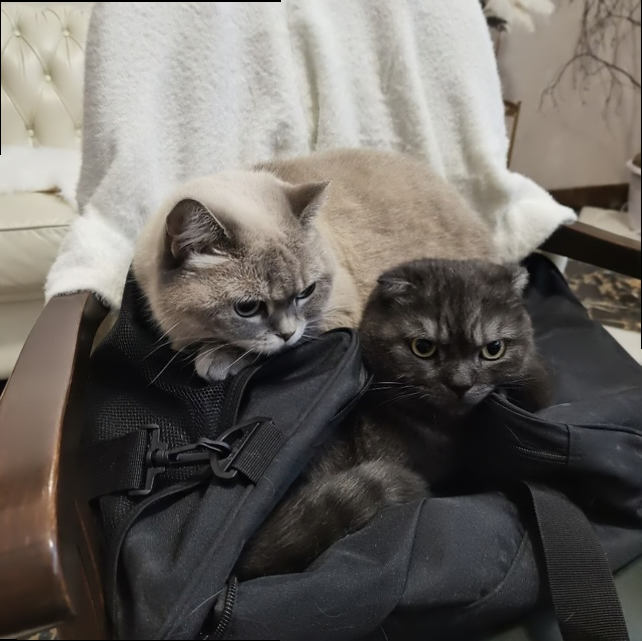
\includegraphics[scale=0.3]{auto_join.png}
        \captionsetup{skip=0pt}
        \caption{Автоматическая склейка кошек}
        \label{Рис:28}
    \end{minipage}
\end{figure}


\section{Ответы на вопросы}
\subsection{Каким образом можно выполнить поворот изображения, не используя матрицу поворота?}
\noindent Самый простой способ -- воспользоваться методом rotate(image, par) из библиотеки OpenCV.
image -- изображение, которое необходимо повернуть, а par -- поворот на сколько и в какую сторону.
Например, в par можно передать cv2.ROTATE\_{90}\_{CLOCKWISE}, cv2.ROTATE\_{90}\_{COUNTERCLOCKWISE}, cv2.ROTATE\_{180},
чтобы повернуть на 90 по часовой стрелке, против и на 180 соответственно


\subsection{Какое минимальное количество соответствующих пар точек необходимо задать на исходном и искаженном изображениях, если порядок преобразования n = 4?}
\noindent Мы можем расчитать это по следующей формуле:
\begin{align*}
    t_{min}=\dfrac{\left(\left(n+1\right)\right)\left(n+2\right)}{2}=\dfrac{\left(\left(4+1\right)\right)\left(4+2\right)}{2}=\dfrac{5\cdot6}{2}=15
\end{align*}


\noindent Таким образом, необходимо передать минимум 15 пар точек


\subsection{После геометрического преобразования изображения могут появиться пиксели с неопределенными значениями интенсивности. С чем это связано и как решается данная проблема?}
\noindent Такое происходит при вращении изображения не на $90^{\circ}$. Есть несколько методов уточнения неопределенных пикселей:
\begin{align*}
    & 1. \text{ Прямой метод}\\
    & \,\,\,\,\,\,\,\,\,\,(a)\text{ Для каждого пикселя вычисляются новые координаты}\\
    & \,\,\,\,\,\,\,\,\,\,(b)\text{ Округляются до ближайших целых значений}\\
    & \,\,\,\,\,\,\,\,\,\,(c)\text{ Неопределенным пикселям нового изображения присваивается яркость}\\
    & \,\,\,\,\,\,\,\,\,\,\,\,\,\,\,\,\,\,\,\,\text{ближайшего после геометрического преобразования пикселя с неокругленными координатами}\\
    & 2. \text{ Обратный метод}\\
    & \,\,\,\,\,\,\,\,\,\,(a)\text{ Координаты каждого пикселя преобразованного изображения подвергаются}\\
    & \,\,\,\,\,\,\,\,\,\,\,\,\,\,\,\,\,\,\,\,\text{обратному преобразованию в систему координат исходного изображения}\\
    & \,\,\,\,\,\,\,\,\,\,(b)\text{ Координаты округляются до ближайших целых значений}\\
    & \,\,\,\,\,\,\,\,\,\,(c)\text{ Берется яркость пикселя с такими координатами}
\end{align*}


\section{Выводы}
\subsection{Лабораторная работа 2}
\noindent В ходе проделанной работы мы познакомились с различными
матричными преобразованиями изображений, начиная с простых эффектов, продолжая
коррекцией дисторсий и заканчивая склеиванием картинок. Мы расширили свои познания
о работе с библиотекой OpenCV и языком программирования python, а также поразмыслили
над интересными вопросами и дали на них ответы
\end{document}